\section{The Exact \texorpdfstring{$5/24$}{5/24} First-Hit Cover}\label{sec:cover}

This section determines the minimum number of upper-half elements needed to
hit every lower-half element by divisibility.

\begin{theorem}[First-hit cover constant]\label{thm:five-twenty-four}
Let
\[
  \tau(n):=\min\{|C|:\ C\subseteq\U_n,\ \forall x\in L_n\ \exists u\in C
  \text{ with }x\mid u\}.
\]
Then
\[
  \tau(n)=\frac{5}{24}n+O(1).
\]
More precisely, the cover
\[
  H_n=\{u\in\U_n:\ u\equiv2\pmod4\}
  \cup
  \{u\in\U_n:\ u>2n/3,\ u\equiv0\pmod4\}
\]
has size $5n/24+O(1)$, and there is a matching packing of lower-half
witnesses of the same size up to $O(1)$.
\end{theorem}

See \Cref{fig:cover-5-24} for the explicit construction.

\begin{figure}[!htbp]
\centering
\begin{tikzpicture}[scale=1.0, xscale=0.55]
  % x-axis: u from n/2 to n, rescaled to [0, 12]
  \draw[thick] (0, -0.5) -- (12, -0.5);
  \foreach \x/\l in {0/{$n/2$}, 4/{$2n/3$}, 12/{$n$}} {
    \draw (\x, -0.45) -- (\x, -0.55);
    \node[below, font=\scriptsize] at (\x, -0.55) {\l};
  }

  % Four residue-class bands, top to bottom: r = 0, 1, 2, 3 (mod 4)
  \foreach \y/\r in {3/{$\equiv 0 \pmod 4$}, 2/{$\equiv 1 \pmod 4$}, 1/{$\equiv 2 \pmod 4$}, 0/{$\equiv 3 \pmod 4$}} {
    \draw[thick] (0, \y) rectangle (12, \y + 0.8);
    \node[left, font=\scriptsize] at (0, \y + 0.4) {\r};
  }

  % Cover piece 1: all u \equiv 2 (mod 4)
  \fill[blue!25] (0, 1.05) rectangle (12, 1.75);
  \node[font=\footnotesize] at (6, 1.4) {cover piece 1};

  % Cover piece 2: u > 2n/3 and u \equiv 0 (mod 4)
  \fill[blue!25] (4, 3.05) rectangle (12, 3.75);
  \node[font=\footnotesize] at (8, 3.4) {cover piece 2: $u > 2n/3$};

  % Annotation of total
  \node[below, font=\small] at (6, -1.4) {$|H_n| = \tfrac{5n}{24} + O(1)$};
\end{tikzpicture}
\caption{The exact first-hit cover $H_n$ from \Cref{thm:intro-cover}.
Upper-half elements are stratified by residue mod $4$. The cover consists
of all $u \equiv 2 \pmod 4$ (entire band) together with $u \equiv 0 \pmod 4$
restricted to $u > 2n/3$ (right portion of the $\equiv 0$ band). Residue
classes $\equiv 1$ and $\equiv 3$ are odd and require no cover element
beyond their own presence. The matching lower-half packing (not shown)
gives $\tau(n) = 5n/24 + O(1)$.}
\label{fig:cover-5-24}
\end{figure}

\begin{proof}
We prove matching upper and lower bounds.

For the upper bound, define
\[
  H_n
  :=
  \{u\in\U_n:\ u\equiv2\pmod4\}
  \cup
  \{u\in\U_n:\ u>2n/3,\ u\equiv0\pmod4\}.
\]
We show that every $x\in L_n$ divides some element of $H_n$.

If $x>n/3$, then $2x\in\U_n$.  If $x$ is odd, then $2x\equiv2\pmod4$; if
$x$ is even, then $2x\equiv0\pmod4$ and $2x>2n/3$.  Hence $2x\in H_n$.

If $n/4<x\le n/3$, then for odd $x$ the element $2x$ lies in $\U_n$ and is
$2$ modulo $4$.  For even $x$, the element $3x$ satisfies
$3x>3n/4>2n/3$ and $3x\le n$; it is even, and is therefore either $2$ or $0$
modulo $4$, with the latter case covered by the condition $3x>2n/3$.  Thus
$3x\in H_n$.

If $n/6<x\le n/4$, then $4x\in\U_n$, $4x>2n/3$, and $4x\equiv0\pmod4$, so
$4x\in H_n$.

Finally suppose $x\le n/6$.  The interval
\[
  \left(\frac{2n}{3x},\frac nx\right]
\]
has length $n/(3x)\ge2$, and hence contains an even integer $k$.  Then
$u=kx$ satisfies $2n/3<u\le n$ and is even.  If $u\equiv2\pmod4$ then
$u\in H_n$ by the first clause; if $u\equiv0\pmod4$ then $u\in H_n$ by the
second clause.  In either case $x\mid u$.

The two clauses defining $H_n$ are disjoint.  Therefore
\[
  \begin{aligned}
  |H_n|
  &=
  \#\{u\in(n/2,n]:u\equiv2\pmod4\} \\
  &\qquad+
  \#\{u\in(2n/3,n]:u\equiv0\pmod4\} \\
  &=
  \frac n8+\frac n{12}+O(1)
  =
  \frac{5n}{24}+O(1).
  \end{aligned}
\]
Thus $\tau(n)\le 5n/24+O(1)$.

For the lower bound, define
\[
  P_n
  :=
  \{m:\ n/3<m\le n/2\}
  \cup
  \{m:\ n/4<m\le n/3,\ m\ \text{odd}\}.
\]
Then
\[
  |P_n|=\frac n6+\frac12\left(\frac n3-\frac n4\right)+O(1)
  =
  \frac{5n}{24}+O(1).
\]

The set $P_n$ is an antichain.  Indeed, if $x<y$ and $x\mid y$, then
$y\ge2x$.  If $y\le n/3$, then $x\le n/6<n/4$, impossible for
$x\in P_n$.  If $n/3<y\le n/2$, then $x\le n/4$, again impossible for
$x\in P_n$.

We claim that any $u\in\U_n$ is divisible by at most one element of $P_n$.
If $x\in P_n$ divides $u$, then $x>n/4$ and $u\le n$, so
\[
  1<\frac ux<4.
\]
Thus $u/x$ is either $2$ or $3$.  If two distinct elements of $P_n$ divide
$u$, they must be $u/2$ and $u/3$.  In particular $6\mid u$.  But then
$u/3$ is even.  It cannot lie in the first component $(n/3,n/2]$ because
$u/3\le n/3$, and it cannot lie in the second component because that component
requires oddness.  Hence at most one element of $P_n$ divides $u$.

Now let $C\subseteq\U_n$ be any cover of $L_n$.  Each $x\in P_n$ must divide
some element of $C$, and the preceding paragraph shows that different
$x\in P_n$ require different elements of $C$.  Therefore
\[
  |C|\ge |P_n|=\frac{5n}{24}+O(1).
\]
This proves the matching lower bound.
\end{proof}
